\chapter*{2 Versuchsdurchführung und Auswertung}
\addcontentsline{toc}{chapter}{2 Versuchsdurchführung und Auswertung}
\setcounter{chapter}{2}
\setcounter{section}{0}
\setcounter{subsection}{0}

\section{Versuch 1: Frequenz und Dämpfung der freien Schwingung}

    \subsection{Versuchsaufbau und -durchführung}

        \begin{figure}[H]
            \centering
            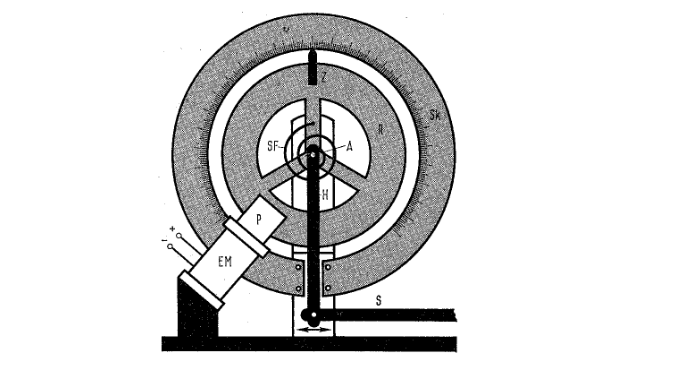
\includegraphics[width=\textwidth]{bilder/aufbau_v1.png}
            \caption{Versuchsaufbau für Versuch 1}
            \label{fig:Aufbau1}
        \end{figure}

        Das Drehpendel in \ref{fig:Aufbau1} besteht aus einer horizontalen Achse (A) einem darum drehenden Kupferring (R), der über eine Spiralfeder (SF) mit einem Hebel (H) verbunden ist und über eine Stange (S) in Bewegung versetzt werden kann. Die Amplitude kann an einer festen Skala (Sk) abgelesen werden. Die Dämpfung wird durch eine Spannungsquelle erzeugt, die über einen Elektromagneten (EM) auf den Kupferring wirkt.
    
        \subsubsection{Teil 1: Eigenfrequenz}
        
            Im ersten Teil von Versuch 1 soll die Eigenfrequenz des Drehpendels bestimmt werden. Der Aufbau ist in \ref{fig:Aufbau1} zu sehen. Um die Eigenfrequenz zu bestimmen wird die Schwingungsdauer wird mit einer Stoppuhr gemessen. Die Messung wird 5 mal wiederholt und läuft über 10 Perioden.
            Die Messergebnisse sind in Tabelle \ref{tab:Eigenfrequenz} zu sehen.    

        \subsubsection{Ergebnisse \& Diskussion}

            \begin{table}[H]
                \centering
                \caption{Messergebnisse Eigenfrequenz}
                \vspace{0.5em}
                \begin{tabular}{|l|l|l|}
                    \hline
                    $n$ & Schwingungsdauer in $\mathrm{s}$ & Periodendauer $T$ in $\mathrm{s}$\\
                    \hline
                    \hline
                    $1$ & $19,27$ & $1,927$ \\
                    \hline
                    $2$ & $19,16$ & $1,916$ \\
                    \hline
                    $3$ & $19,20$ & $1,920$ \\
                    \hline
                    $4$ & $18,95$ & $1,895$ \\
                    \hline
                    $5$ & $19,11$ & $1,911$ \\
                    \hline
                \end{tabular}
                \label{tab:Eigenfrequenz}
            \end{table}

            Da die Schwingungdauer über 10 Perioden gemessen wird um den Messfehler so gering wie möglich zu halten, muss der Messwert durch $10$ geteilt werden um die Periodendauer zu erhalten. Der Fehler lässt sich auf die Reaktionszeit des Menschen zurückführen und darauf das die Stoppuhr 2 mal betätigt werden muss. Da der Fehler bei der Messung der Schwingungsdauer betrachtet werden muss, wird der Fehler für die Periodendauer ebenfalls durch 10 geteilt.
            Man erhält nun einen Mittelwert für die Periodendauer von $T = 1,914 \pm 0,06\ \mathrm{s}$. Die $0,06$ basieren auf der 2-fachen Reaktionszeit des Menschen: \url{https://de.wikipedia.org/wiki/Reaktion_(Verkehrsgeschehen)}.
            Die Eigenfrequenz können wir nun mit folgender Formel berechnen:

            \begin{equation}
                f = \frac{1}{T}
                \label{eq:Frequenz}
            \end{equation}

            Daraus resultiert eine Eigenfrequenz von:

            \begin{equation}
                \omega_{0} = 2 \pi \cdot f = 2 \pi \cdot \frac{1}{T} = 2 \pi \cdot \frac{1}{1,914\ \mathrm{s}} = 3,28\ \mathrm{Hz}
                \label{eq:Eigenfrequenz}
            \end{equation}

            Nun können wir noch den geforderten Größtfehler $\Delta \omega_{0}$ berechnen. Dazu verwenden wir folgende Formeln:

            \begin{equation}
                \begin{aligned}
                \Delta f &= f \cdot \frac{\Delta T}{T}\\
                \Delta \omega_{0} &= \left|2 \pi \cdot -\frac{1}{T^{2}} \cdot \Delta T\right|
                \end{aligned}
                \label{eq:Größtfehler}
            \end{equation}

            Wir erhalten einen Größtfehler von $\Delta \omega_{0} = 0,10\ \mathrm{Hz}$ und somit eine Eigenfrequenz von $\omega_{0} = (3,28 \pm 0,10)\ \mathrm{Hz}$.

            Das Ergebnis lässt sich nun diskutieren. Da wir keinen Literaturwert haben, können wir nur die Messwerte betrachten. Diese sind in Tabelle \ref{tab:Eigenfrequenz} zu sehen. Die Messwerte sind sehr nah beieinander lässt also darauf schließen, dass hier eine gewisse Konsistenz vorhanden ist. Allerdings ist das Drehpendel nicht ideal, was die Varianz erklärt. Das Endergebnis ist also durchaus plausibel. Zudem kommt, dass eine natürliche Dämpfung vorhanden ist, die die Schwingungsdauer beeinflusst. Diese wurde hier nicht berücksichtigt, weshalb die Messwerte nicht exakt gleich sind.

        \subsubsection{Teil 2: Dämpfung}
        
            Im zweiten Teil soll die Dämpfung des Drehpendels bestimmt werden. Der Versuchsaufbau ist auch hier in \ref{fig:Aufbau1} zu sehen. Im Unterschied zu Teil 1 wird nun allerdings eine Dämpfungsspannung von $2\ \mathrm{V}$, bzw. $4\ \mathrm{V}$ angelegt. Wir möchten hier nun die Dämpungskonstante $\beta$ sowie das Dämpfungsverhältnis $K$ bestimmen. Letzteres beschreibt die relative Veränderung der Amplitude pro Periode. Die Dämpfungskonstante lässt sich nun mit folgender Formel\footnote[1]{Die Formel wurde in der Anleitung des Versuchs hergeleitet und von uns übernommen.} berechnen:

            \begin{equation}
                \beta = \frac{\ln K}{T}
                \label{eq:Dämpfungskonstante}
            \end{equation}

            Die Messung der Amplitude und der Periodendauer erfolgt in zwei Teilen. Das liegt daran, dass die Periodendauer unabhängig von der Amplitude, im Idealfall, immer gleich bleibt. Die Amplitude wird an der Skala des Drehpendels abgelesen. Die Messung der Periodendauer erfolgt über eine weitere Messung, die später noch erläutert wird. Die Messergebnisse sind in Tabelle \ref{tab:ergebnisse_v1.2} zu sehen.

            %Desweiteren ist zu beachten, dass sich das Drehpendel auf der rechten Seite anders verhält als auf der linken, deshalb wurden die Amplituden getrennt voneinander bestimmt. Insgesamt wurde pro Dämpfungsspannung 3 mal mit gleicher Anfangsauslenkung jede Seite gemessen.

        \subsubsection{Ergebnisse \& Diskussion}

            Man erhält nun folgenden Werte für die Dämpfung $\beta$:
            Fehler in der Tabelle nicht vergessen
            
            \begin{table}[H]
                \centering
                \caption{Dämpfung bei $2\ \mathrm{V}$ und $4\ \mathrm{V}$}
                \vspace{0.5em}
                \begin{tabular}{|l|l|l||l|l|}
                    \hline
                    $n$ & Zeit $t$ in $\mathrm{s}$ bei $2\ \mathrm{V}$ & Amplitude bei $2\ \mathrm{V}$ & Zeit $t$ in $\mathrm{s}$ bei $4\ \mathrm{V}$ & Amplitude bei $4\ \mathrm{V}$\\
                    \hline
                    \hline
                    $0$ & $0,000$ & $17,0$ & $0,000$ & $17,0$ \\
                    \hline
                    $1$ & $1,946$ & $14,2$ & $1,945$ & $9,2$ \\
                    \hline
                    $2$ & $3,892$ & $12,0$ & $3,890$ & $5,0$ \\
                    \hline
                    $3$ & $5,838$ & $10,0$ & $5,835$ & $2,6$ \\
                    \hline
                    $4$ & $7,784$ & $8,4$ & $7,78$ & $1,4$ \\
                    \hline
                    $5$ & $9,730$ & $7,2$ & $9,725$ & $1,0$ \\
                    \hline
                    $6$ & $11,676$ & $6,0$ & $11,670$ & $0,6$ \\
                    \hline
                    $7$ & $13,622$ & $5,0$ & $13,615$ & $0,4$ \\
                    \hline
                    $8$ & $15,568$ & $4,0$ & - & - \\
                    \hline
                    $9$ & $17,514$ & $3,4$ & - & - \\
                    \hline
                \end{tabular}
                \label{tab:ergebnisse_v1.2}
            \end{table}

            Die folgenden zwei Graphen \ref{fig:plot_v1_2V} und \ref{fig:plot_v1_4V} zeigen die Messwerte aus Tabelle \ref{tab:ergebnisse_v1.2} in einem Diagramm. Die Funktionsgleichung wurde mit einem Fit bestimmt, welcher durch die rote Trendlinie dargestellt wird.
            
            \begin{figure}[H]
                \begin{subfigure}{0.48\textwidth}
                    \centering
                    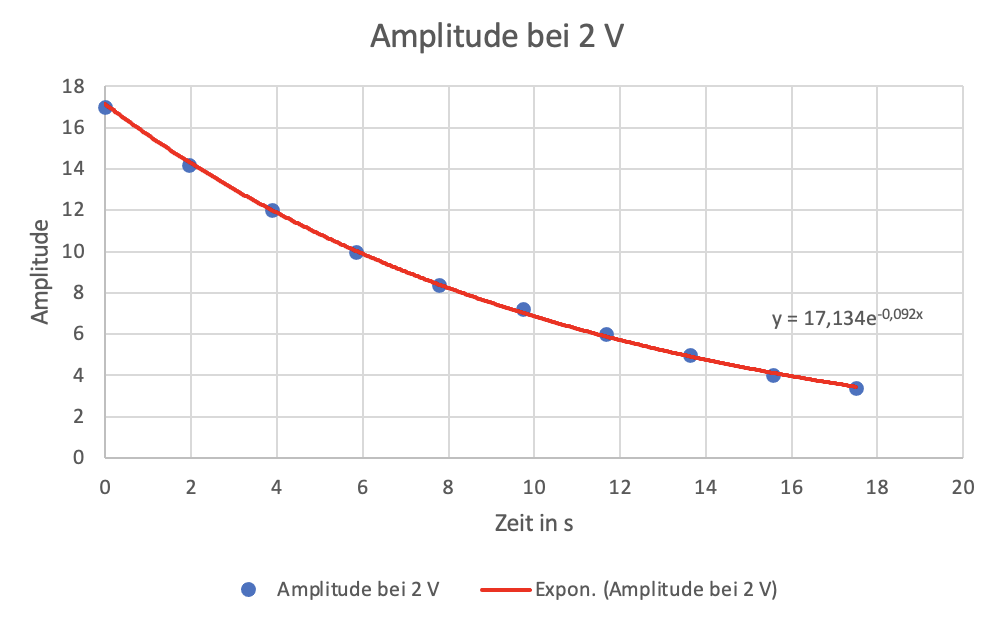
\includegraphics[width=\textwidth]{bilder/plot_v1_2V.png}
                    \caption{Amplitude bei $2\ \mathrm{V}$}
                    \label{fig:plot_v1_2V}
                \end{subfigure}
                \begin{subfigure}{0.48\textwidth}
                    \centering
                    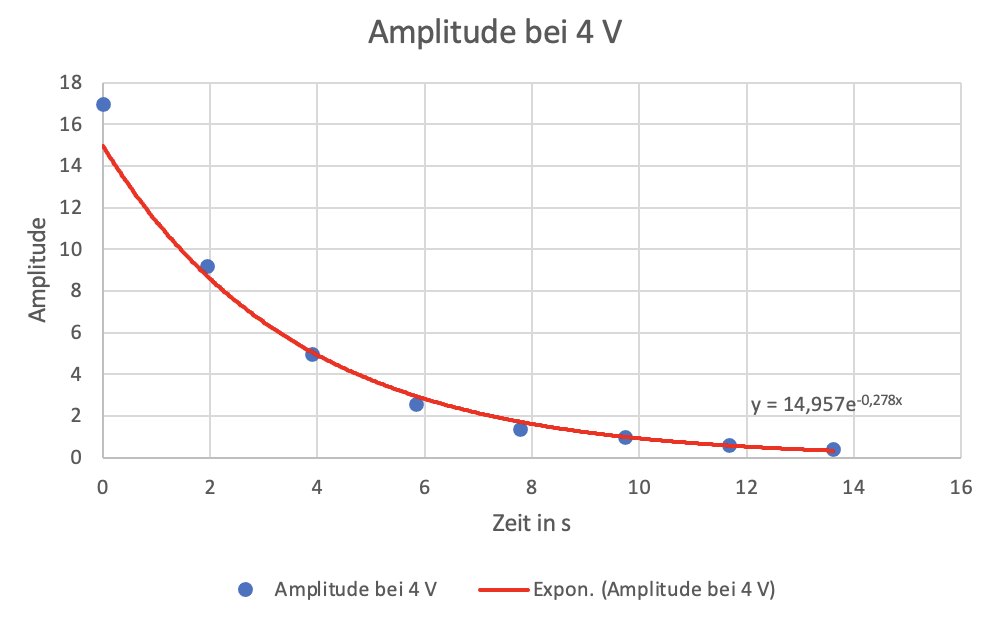
\includegraphics[width=\textwidth]{bilder/plot_v1_4V.png}
                    \caption{Amplitude bei $4\ \mathrm{V}$}
                    \label{fig:plot_v1_4V}
                \end{subfigure}
            \end{figure}

            Wie bereits oben erwähnt, wurde die Periodendauer über eine weitere Messung bestimmt. Das Drehpendel besitzt eine Zeitschranke, welche bei Amplitude $0$ angebracht ist. Um nun die Amplitude zu messen, wird das Drehpendel ausgelenkt und die Zeit gemessen, die das Pendel für eine Auslenkung auf einer Seite des Nullpunktes benötigt. Die Messung wird für beide Seiten durchgeführt, da die Zeitschranke nicht perkekt symmetrisch ist. Die Werte werden addiert.

            Final können wir nun $\beta$ und $K$ bestimmen. Für $\beta$ gibt es zwei Wege. Der erste Weg ist einfach, da die Berechnung von Excel getätigt wurde. Die Funktionen der Fits \ref{fig:plot_v1_2V} und \ref{fig:plot_v1_4V} beinhalten bereits den finalen Wert. Der zweite Weg ist die Berechnung mit der Formel \ref{eq:Dämpfungskonstante}. Hierzu muss die Dämpfungskonstante bestimmt werden. Diese wird durch das Verhältnis der Amplituden bestimmt. Wir verwenden die Werte von $n = 1$ und $n = 2$ aus Tabelle \ref{tab:ergebnisse_v1.2}.

            Die Ergebnisse sind in folgender Tabelle \ref{tab:ergebnisse_v1.2_final} zu sehen.

            \begin{table}[H]
                \centering
                \caption{Ergebnisse für $\beta$ und $K$}
                \vspace{0.5em}
                \begin{tabular}{|l|l|l|l|}
                    \hline
                    Dämpfungsspannung & $\beta_{1}$& $\beta_{2}$ & $K$\\
                    \hline
                    \hline
                    $2\ \mathrm{V}$ & $0,092$ & $0,087$ & $1,18$\\
                    \hline
                    $4\ \mathrm{V}$ & $0,278$ & $0,314$ & $1,84$\\
                    \hline
                \end{tabular}
                \label{tab:ergebnisse_v1.2_final}
            \end{table}

            Da die finalen Ergebnisse von $\beta_{1}$ und $\beta_{2}$ sehr nah beieinander liegen, kann davon ausgegangen werden, dass die Messung recht genau war. Die Werte für $\beta$ im Vergleich zwischen $2\ \mathrm{V}$ und $4\ \mathrm{V}$ sind ebenfalls plausibel. Die Dämpfung ist bei $4\ \mathrm{V}$ größer, was auch zu erwarten war. Allerdings sollte $\beta_{1}$ genauer sein, da dieser alle Messwerte beinhalten und nicht nur zwei.

\newpage

\section{Versuch 2: Computersimulation}

    \subsection{Versuchsaufbau und -durchführung}

        \subsubsection{Teil 1: Erzwungene Schwingungen}
            
            In Teil 1 wird in einer vorbereiteten Matlab-Applikation die Resoanzkurve und damit die Resonanzfrequenz des simulierten Pendels herausgefunden. Die Applikation stellt zwei Diagramme zur Verfügung \ref{fig:plots_v2}. Diese stellen einmal die Amplituden und einmal die Phasen der Schwingung dar.
            
            \begin{figure}[H]
                \centering
                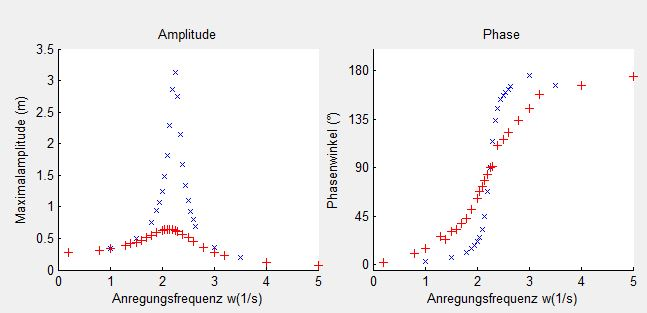
\includegraphics[width=\textwidth]{bilder/plots_v2.jpg}
                \caption{Plots der Applikation für Versuch 2 Teil 1}
                \label{fig:plots_v2}
            \end{figure}

            Es lässt sich gut erkennen, dass die Amplitude des Pendels maximal ist, wenn die Phasenverschiebung der Anregerfrequenz $90\text{\textdegree}$ beträgt.

            \textcolor{red}{TODO: Restliche Fragen beantworten und Masse bestimmen}

        \subsubsection{Teil 2: Infrarotspektroskopie}
        
            Im zweiten Teil wird der Zusammenhang zwischen Infrarotspektroskopie und Molekülschwingungen dargestellt. Das folgende Diagramm \ref{fig:diagram_v2} stellt die verschiedenen Ausschläge bei verschiedenen Wellenzahlen dar.

            \begin{figure}[H]
                \centering
                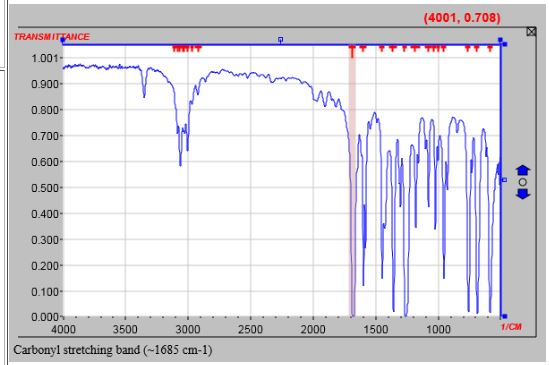
\includegraphics[width=\textwidth]{bilder/diagram_v2.jpg}
                \caption{Diagramm der Applikation für Versuch 2 Teil 2}
                \label{fig:diagram_v2}
            \end{figure}

            Bei einer Wellenzahl von ca. $3070$ bewegen sich die weißen Moleküle. bei einer Wellenzahl von ca. $2998$ bewegen sich die weißen ebenfalls, allerdings in eine andere Richtung. Und bei einer Wellenzahl von ca. $1688$ bewegt sich das Sauerstoffmolekül.

\newpage

\section{Versuch 3: Erzwungene Schwingungen}

    \subsection{Versuchsaufbau und -durchführung}
            
        In Versuch 3 wird der gleiche Aufbau wie in Versuch 1 verwendet: \ref{fig:Aufbau1}. Diesmal wird allerdings der Motor zur Anregung verwendet. Es muss zusätzlich noch eine Dämpfungsspannung von $2\ \mathrm{V}$ angelegt werden, da das Pendel sonst die maximale Amplitude überschreitet. Die Messung der Amplitude erfolgt wie üblich über die Skala des Drehpendels. Die Messung der Periodendauer erfolgt ebenfalls wie in Versuch 1. Teil 2. Die Anregerfrequenz kann am Gerät abgelesen werden und die Phasenzeit wird ebenfalls über eine extra Messung wie die der Amplitude durchgeführt. Hierzu wird das Gerät, welches die Anregerfrequenz erzeugt benutzt, welche einem die Phasenzeit anzeigt.

        \subsubsection{Teil 1: Resonanzfrequenz}
        
            Im ersten Teil soll die Resonanzfrequenz des Drehpendels bestimmt werden. Um die Resonanzfrequenz zu finden wird das Rädchens am Motor solange erhöht, bis eine maximale Amplitude erreicht wird. Die maximale Amplitude des Drehpendels befindet sich bei 10 Skaleneinheiten und bei einer Motor Skalenteilen von 500.

        \subsubsection{Teil 2: Resonanz- und Phasenkurve}
    
            Nun werden alle Messwerte in einem kleinen Umkreis um das Maximum in kleinen Schritten gemessen, und bei weiterem Abstand in größeren Schritten. Die Messwerte sind in Tabelle \ref{tab:ergebnisse_v3} zu sehen.

            Die Messwerte des Motors, der Periodendauer, der Amplitude und der Phasenzeit können dabei ohne weiteres abgelesen werden. Die Anregerfrequenz wird mit der folgenden Formel berechnet:

            \begin{equation}
                \omega_{a} = \frac{2 \pi}{T}
            \end{equation}

            Die Phasenverschiebung Phi wird mit folgender Formel berechnet:

            \begin{equation}
                \varphi = \frac{\text{Phasenzeit}}{T}
            \end{equation}

            \begin{table}[H]
                \centering
                \caption{Messergebnisse für Versuch 3}
                \vspace{0.5em}
                \begin{tabular}{|l|l|l|l|l|l|l|l|}
                    \hline
                    Motor & $\frac{T}{2}$ links in $\mathrm{ms}$ & $\frac{T}{2}$ rechts in $\mathrm{ms}$ & $\mathrm{T}$ in $\mathrm{ms}$ & $\omega_{a}$ in $\frac{1}{\mathrm{s}}$ & Amplitude & $\varphi$ in $\mathrm{ms}$ & Phi in Grad\\
                    \hline
                    \hline
                    $445$ & $1117$ & $1054$ & $2171$ & $2,89$ & $2,4$ & $65$ & $10,78$\\
                    \hline
                    $465$ & $1058$ & $1026$ & $2084$ & $3,01$ & $3,4$ & $122$ & $21,07$\\
                    \hline
                    $475$ & $1034$ & $1015$ & $2049$ & $3,07$ & $4,5$ & $163$ & $28,64$\\
                    \hline
                    $485$ & $1001$ & $1003$ & $2004$ & $3,14$ & $6,4$ & $248$ & $44,55$\\
                    \hline
                    $490$ & $984$ & $998$ & $1982$ & $3,17$ & $8,0$ & $308$ & $55,94$\\
                    \hline
                    $495$ & $971$ & $994$ & $1965$ & $3,20$ & $9,4$ & $397$ & $72,73$\\
                    \hline
                    $500$ & $959$ & $987$ & $1946$ & $3,23$ & $10,0$ & $498$ & $92,13$\\
                    \hline
                    $505$ & $950$ & $974$ & $1924$ & $3,27$ & $9,4$ & $617$ & $115,45$\\
                    \hline
                    $510$ & $946$ & $965$ & $1911$ & $3,29$ & $8,4$ & $667$ & $125,65$\\
                    \hline
                    $515$ & $941$ & $950$ & $1891$ & $3,32$ & $7,0$ & $717$ & $136,50$\\
                    \hline
                    $525$ & $931$ & $924$ & $1855$ & $3,39$ & $4,8$ & $761$ & $147,69$\\
                    \hline
                    $535$ & $923$ & $901$ & $1824$ & $3,44$ & $3,8$ & $777$ & $153,36$\\
                    \hline
                    $555$ & $906$ & $895$ & $1765$ & $3,56$ & $2,4$ & $771$ & $157,26$\\
                    \hline
                \end{tabular}
                \label{tab:ergebnisse_v3}
            \end{table}

            Die folgenden Diagramme \ref{fig:plot_v3_1} und \ref{fig:plot_v3_2} visualisieren die Messwerte aus Tabelle \ref{tab:ergebnisse_v3}.

            \begin{figure}[H]
                \begin{subfigure}{0.48\textwidth}
                    \centering
                    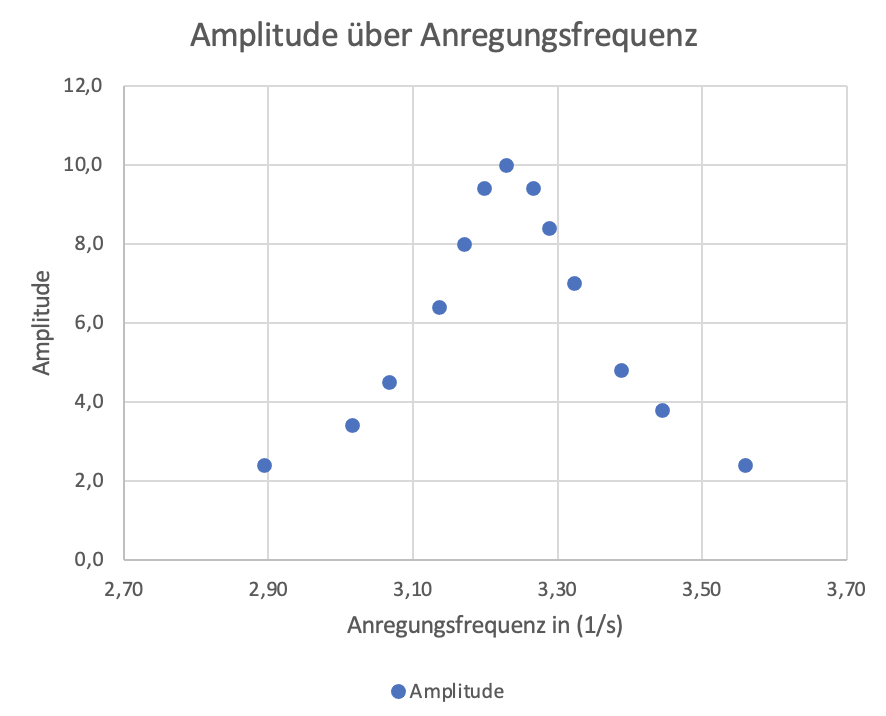
\includegraphics[width=\textwidth]{bilder/plot_v3_1.png}
                    \caption{Amplitude über Anregungsfrequenz}
                    \label{fig:plot_v3_1}
                \end{subfigure}
                \begin{subfigure}{0.48\textwidth}
                    \centering
                    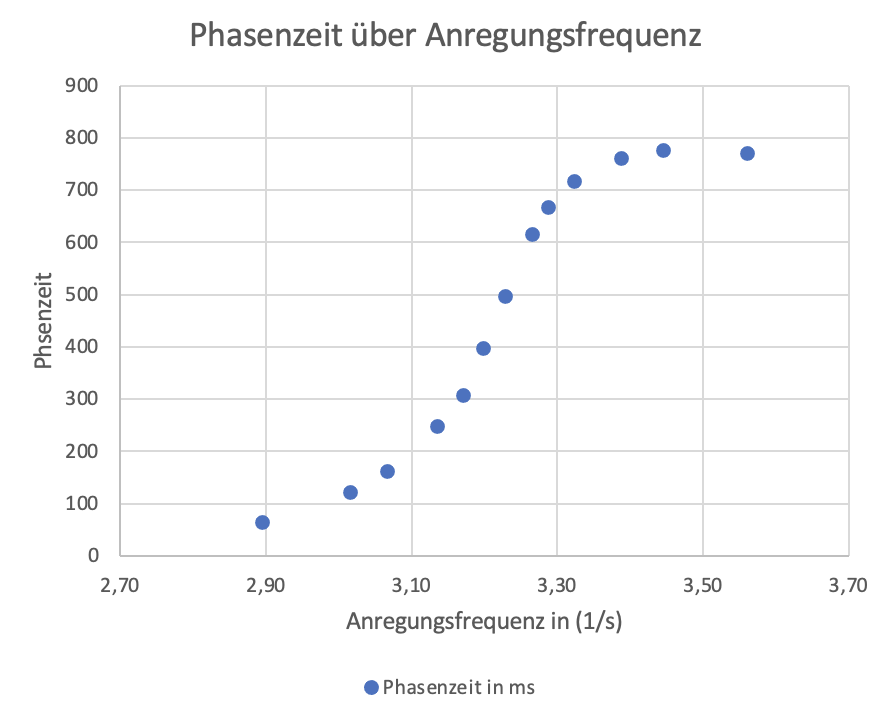
\includegraphics[width=\textwidth]{bilder/plot_v3_2.png}
                    \caption{Phasenzeit über Anregungsfrequenz}
                    \label{fig:plot_v3_2}
                \end{subfigure}
            \end{figure}
        
        \subsubsection{Teil 3: Auswertung der Resonanzkurve}

            Die Ergebnisse wurden nun im Tool Origin ausgewertet und verschiedene Diagramme erstellt:

            \begin{figure}[H]
                \begin{subfigure}{0.48\textwidth}
                    \centering
                    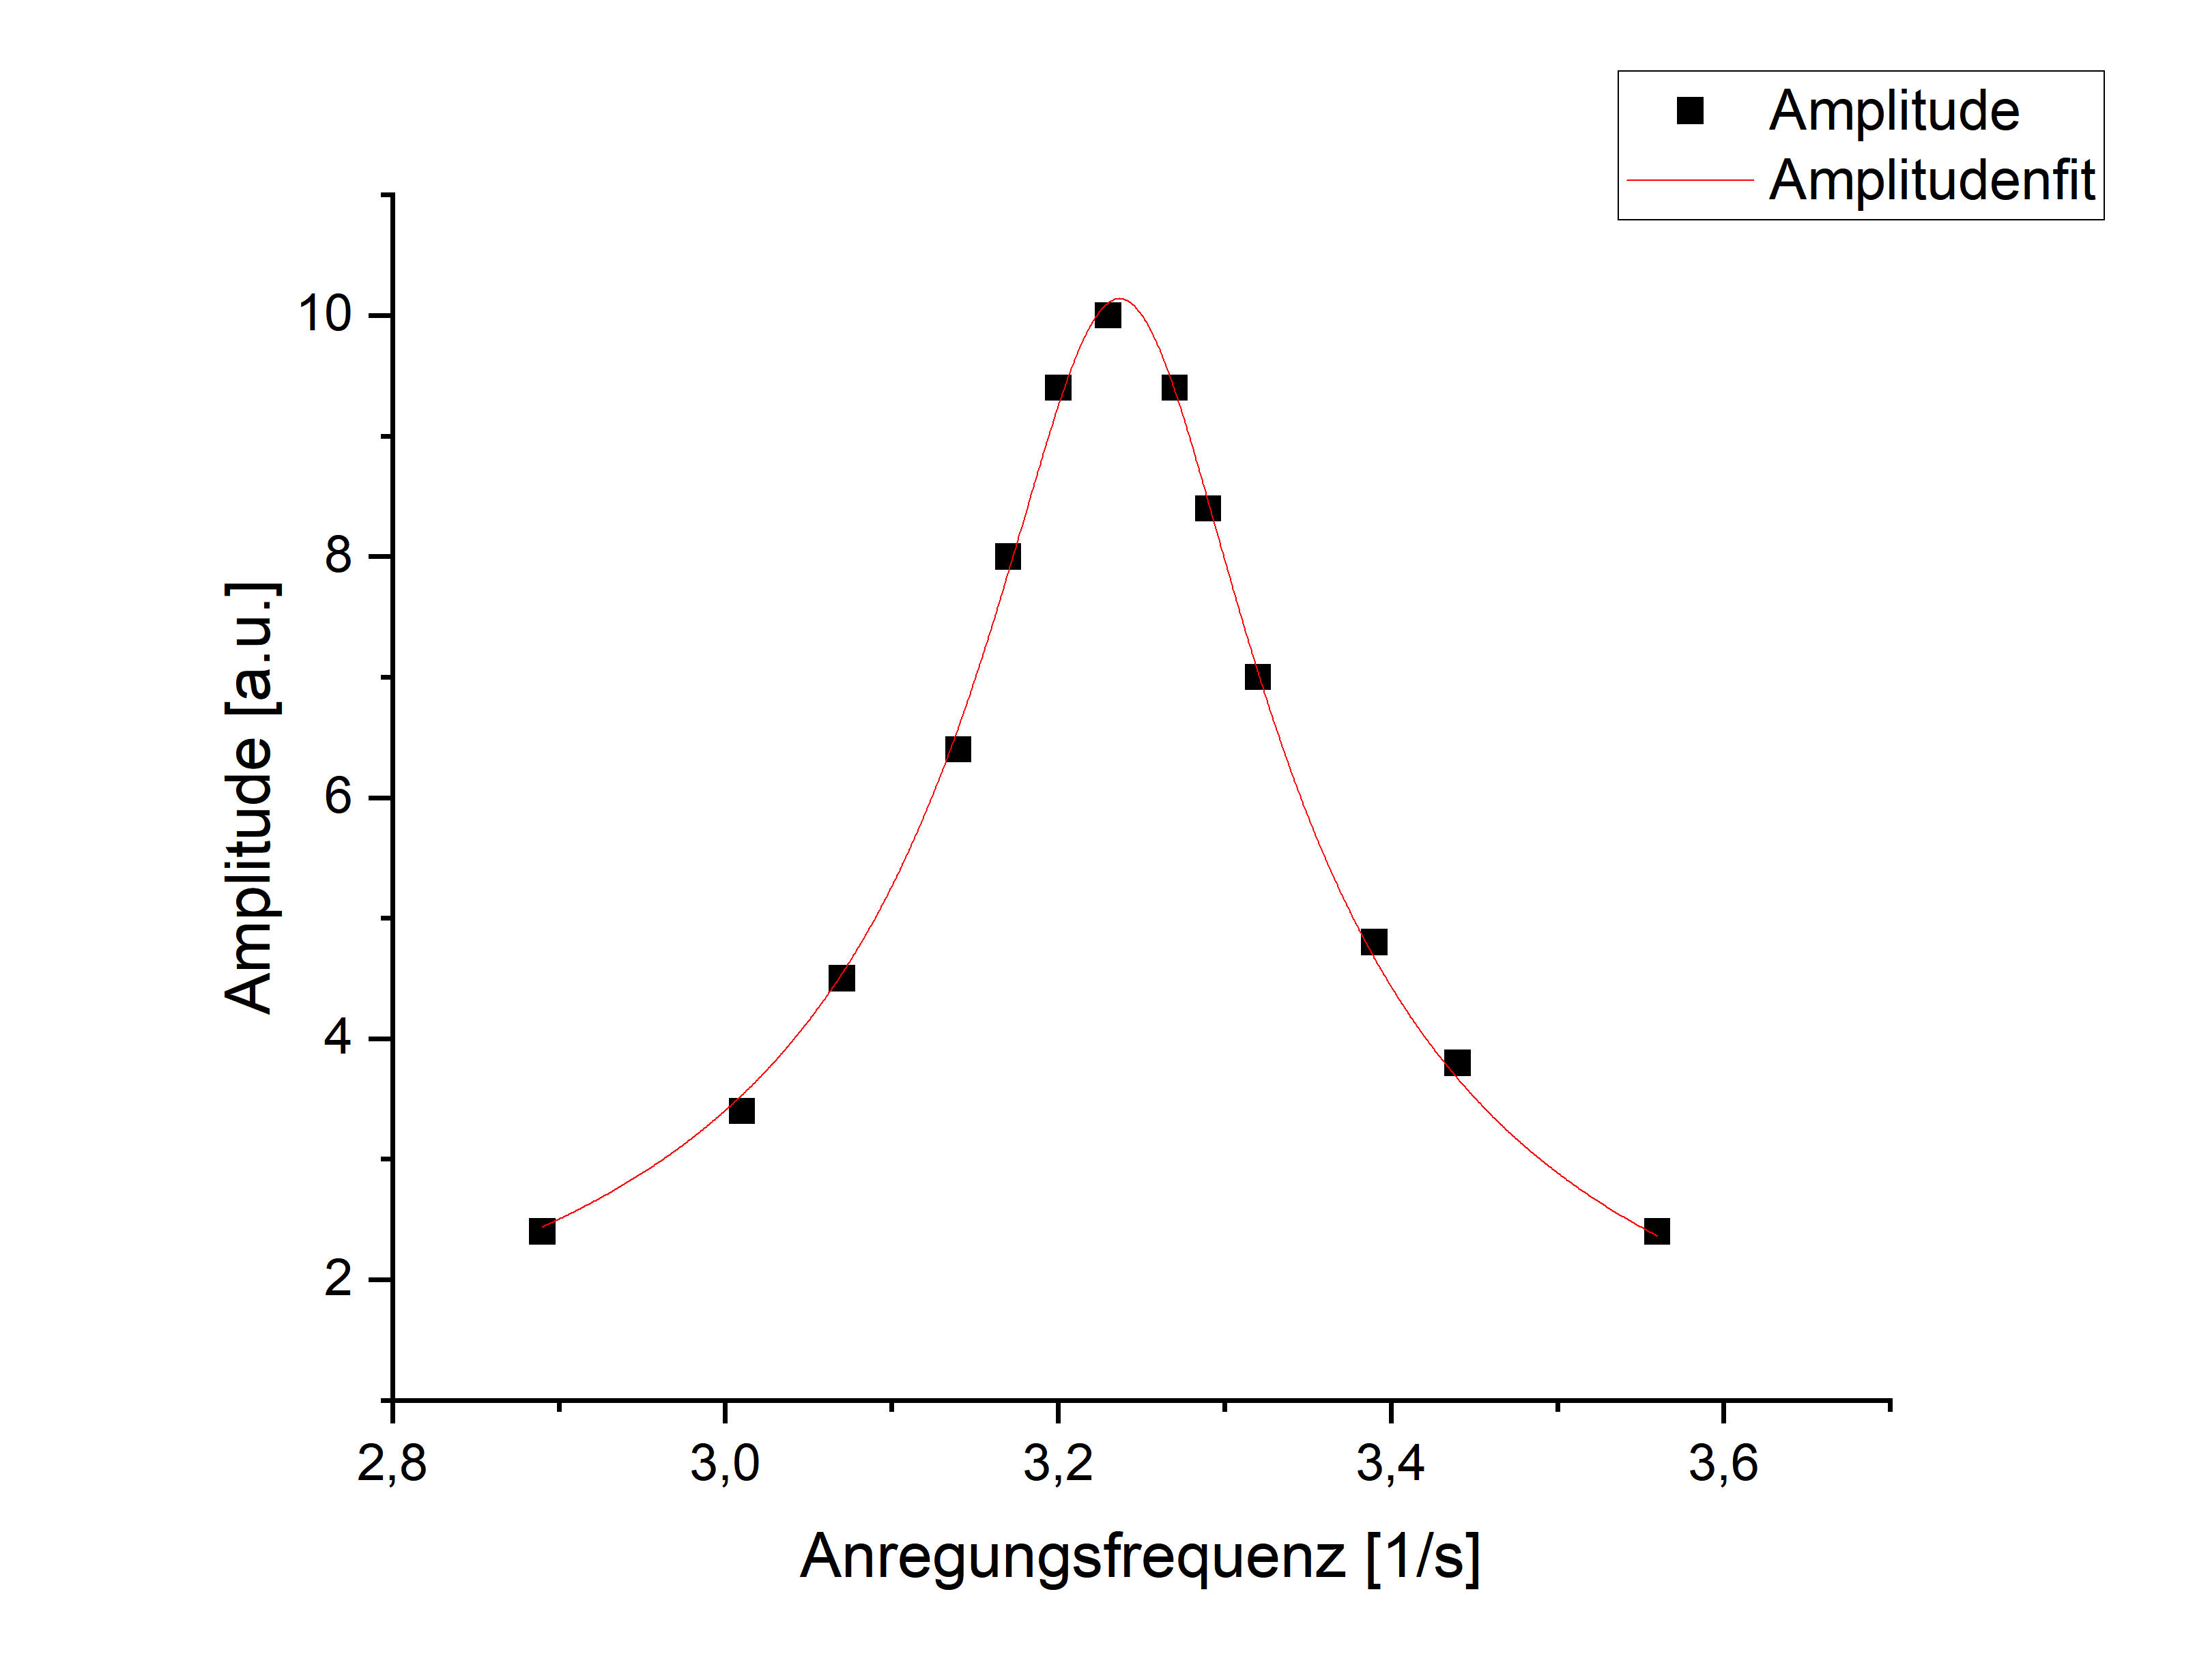
\includegraphics[width=\textwidth]{bilder/AmplitudenkurveGruppe2.png}
                    \caption{Amplitudenkurve}
                    \label{fig:Amplitudenkurve}
                \end{subfigure}
                \begin{subfigure}{0.48\textwidth}
                    \centering
                    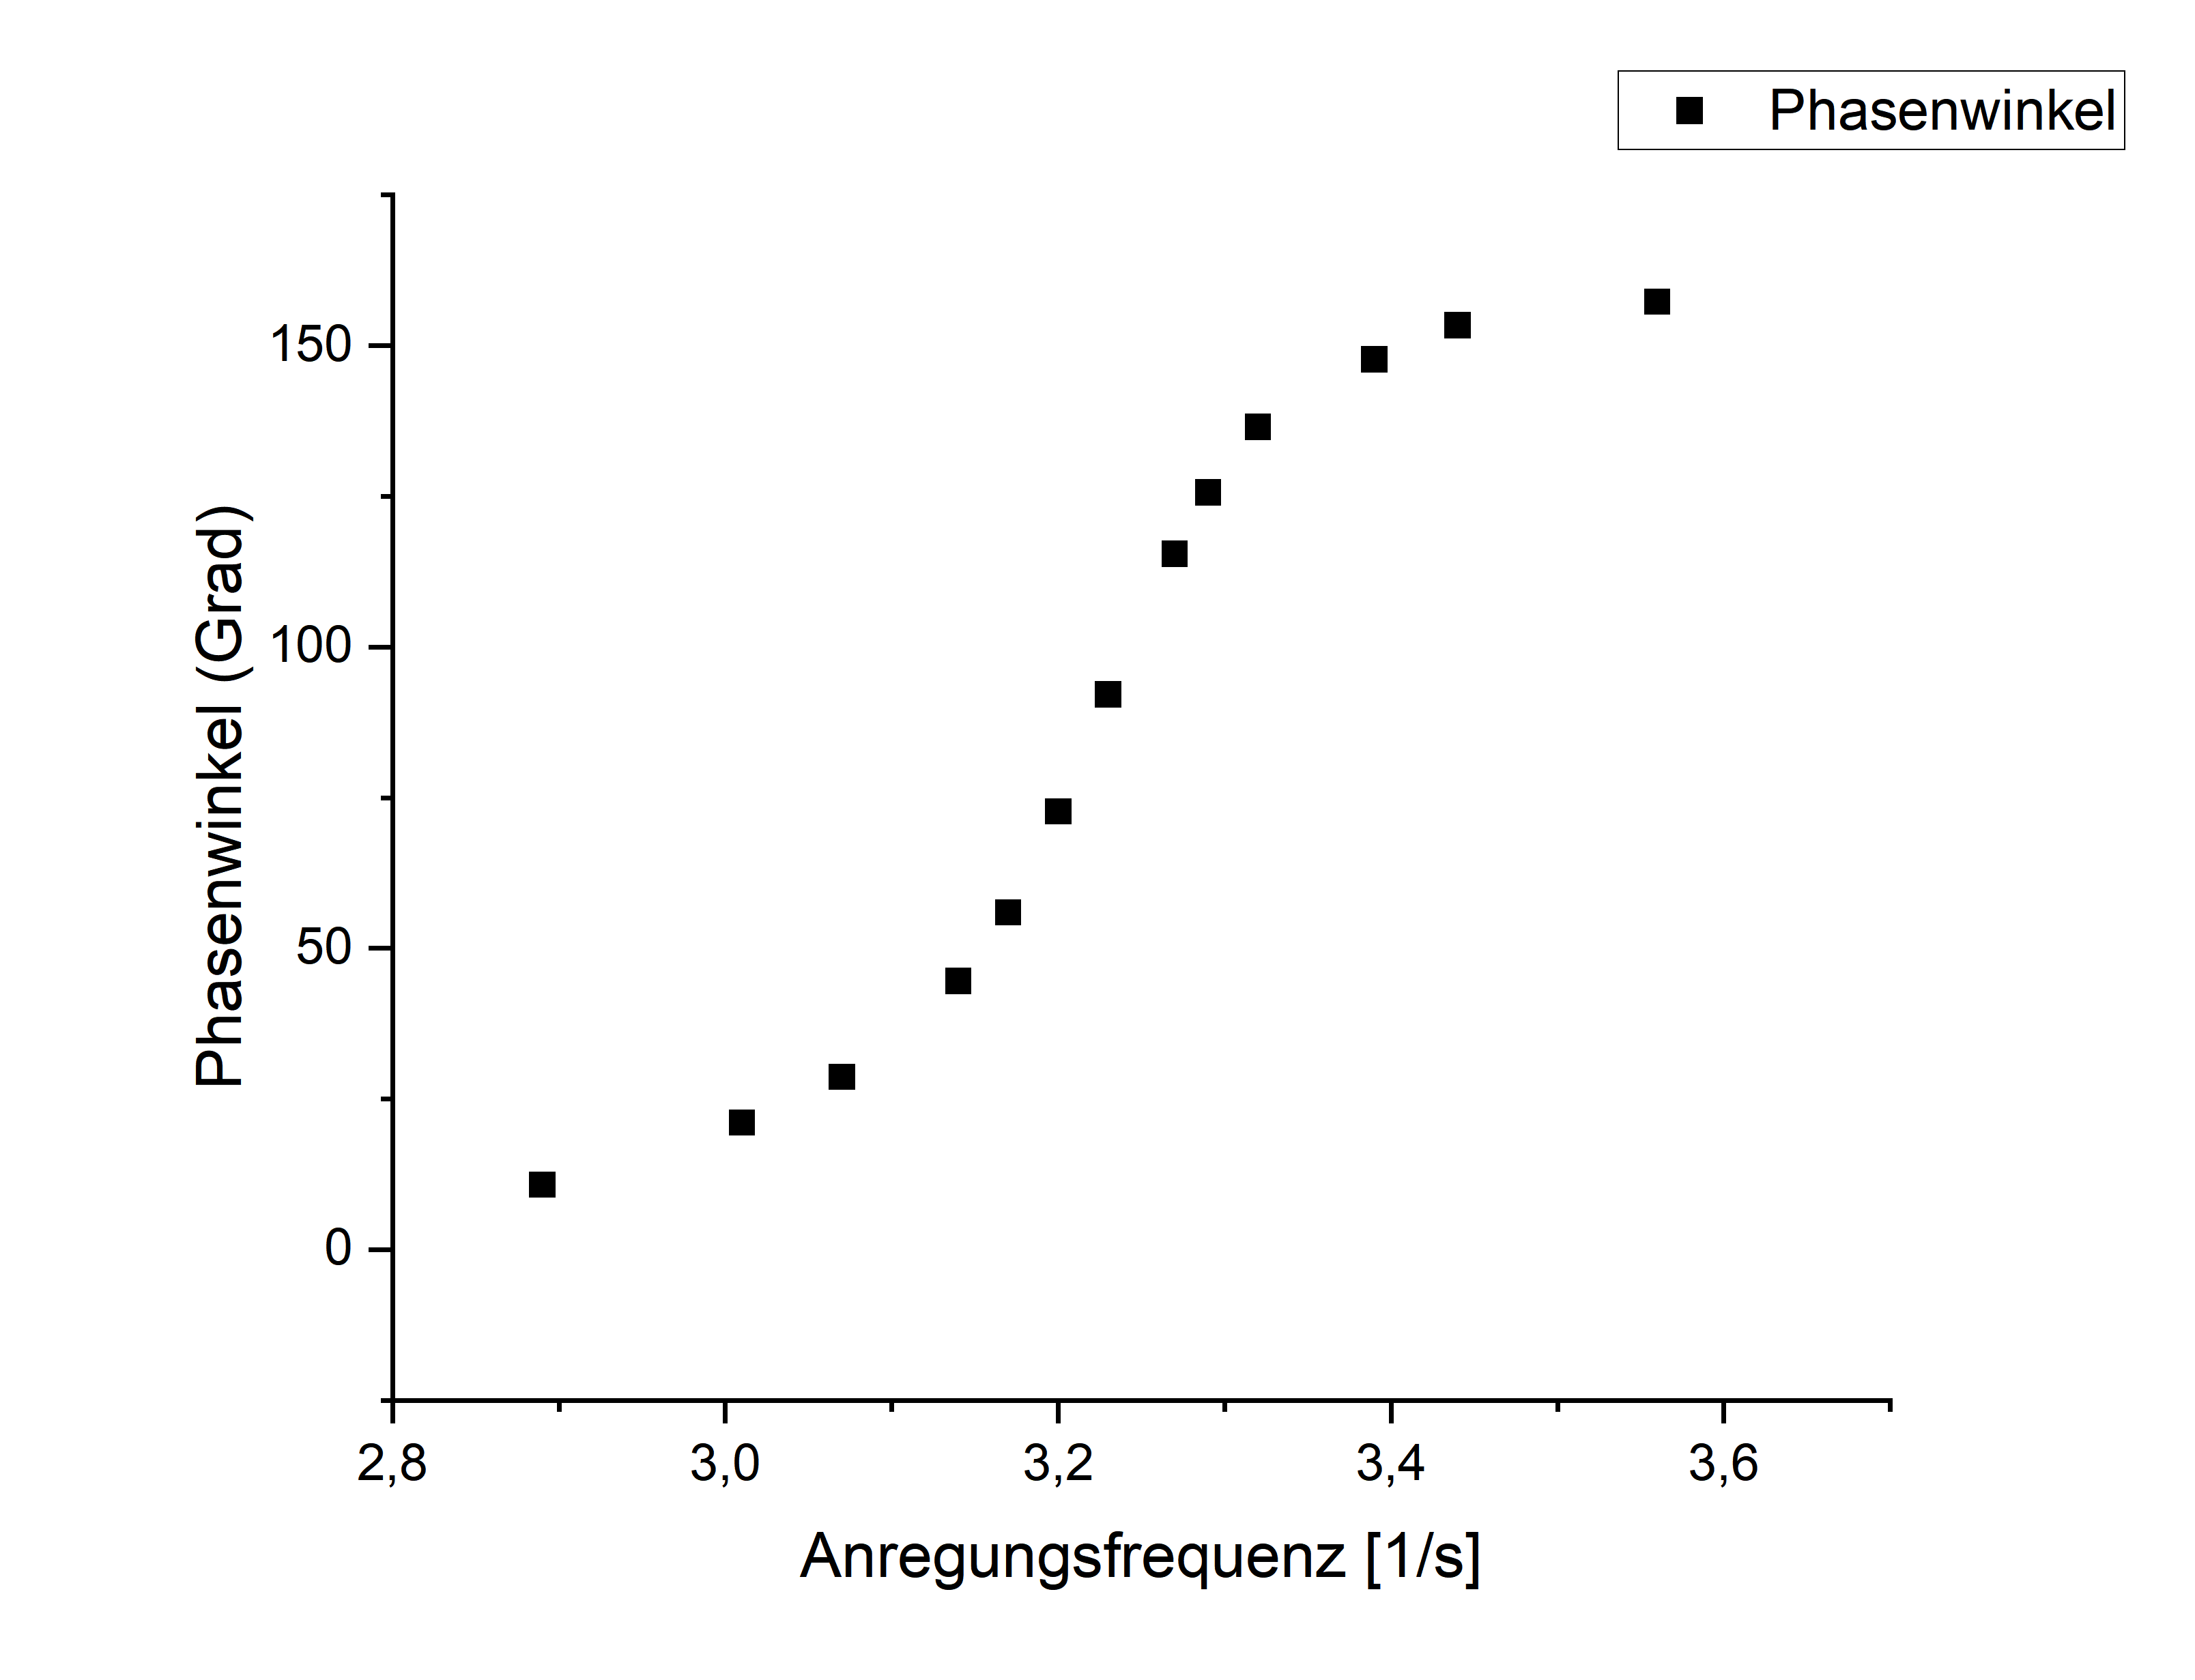
\includegraphics[width=\textwidth]{bilder/PhasenwinkelGruppe2.png}
                    \caption{Phasenkurve}
                    \label{fig:Phasenkurve}
                \end{subfigure}
            \end{figure}

            \begin{figure}[H]
                \centering
                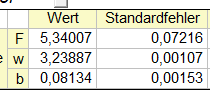
\includegraphics[width=0.25\textwidth]{bilder/fehler_v3.png}
                \caption{Fehler}
                \label{fig:fehler}
            \end{figure}
            
            \textcolor{red}{TODO: Ausschmücken mit Text}

        \subsubsection{Diskussion}
            
            \textcolor{red}{TODO: Diskussion}